\documentclass{article}
\usepackage{multicol}
\usepackage[utf8]{inputenc}
\usepackage{float}
\usepackage{graphicx}
\usepackage{hyperref}
\hypersetup{
    colorlinks=true,
    urlcolor=blue,
    }
    
\usepackage{geometry}
\geometry{
    a4paper,
    total={170mm,257mm}
    }

\usepackage{forest}
\definecolor{folderbg}{RGB}{124,166,198}
\definecolor{folderborder}{RGB}{110,144,169}
\def\Size{4pt}
\tikzset{
  folder/.pic={
    \filldraw[draw=folderborder,top color=folderbg!50,bottom color=folderbg]
      (-1.05*\Size,0.2\Size+5pt) rectangle ++(.75*\Size,-0.2\Size-5pt);  
    \filldraw[draw=folderborder,top color=folderbg!50,bottom color=folderbg]
      (-1.15*\Size,-\Size) rectangle (1.15*\Size,\Size);
  }
}

% ------------------------------- FRONT MATTER ------------------------------- %

\title{\textbf{GreenBook}\\~\\
    Third assignment\\
    \small Software Development Process course\\
        University of Milano - Bicocca\\
        A.A. 2021/22\\~\\
        \href{https://gitlab.com/massimino96/2021_assignment3_greenbook/}{Repository Link}}
\author{Authors:\\
    830260 - Binda Paolo - \href{mailto:p.binda@campus.unimib.it}{p.binda@campus.unimib.it}\\
    831075 - D'Apa Massimo - \href{mailto:m.dapa@campus.unimib.it}{m.dapa@campus.unimib.it}\\
    830065 - Fornaro Alessandro - \href{mailto:a.fornaro1@campus.unimib.it}{a.fornaro1@campus.unimib.it}}
\date{}

% ------------------------------- DOC. START ------------------------------- %

\begin{document}
\setlength{\parindent}{0em}
\setlength{\parskip}{1em}

\maketitle
\thispagestyle{empty}

\cleardoublepage
\setcounter{page}{1}

\section*{Introduction}

Due to the outbreak of the recent COVID-19 pandemic, we found it useful to develop a web-app that would facilitate the traceability of possible infections for managers of clubs and restaurants. In fact, COVID virus can easily spread within a restaurant in the presence of many people in the same closed environment.

GreenBook is a Spring web-app that allows to manage reservations in a restaurant, with a particular focus on the traceability of possible COVID infections thanks to booking records.

\section*{ER Model Design}
\begin{figure}[H]
    \centering
    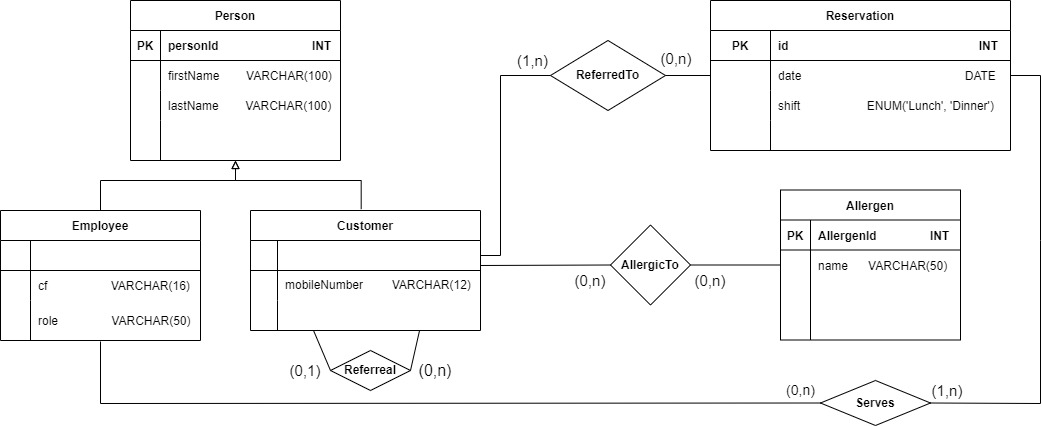
\includegraphics[width=\textwidth]{ER}
    \caption{ER Model}
    \label{fig:ermodel}
\end{figure}

In the phase of ER Design, we made the following assumptions:
\begin{itemize}
  \item A user cannot recommend himself
  \item Tracing also employees which are selected for each reservation should be useful, since they could be infected and, in such cases, we need to be able to track them too
  \item Each customers' credentials are asked during the booking process, so that every person relating to a reservation gets recorded
  \item A restaurant could find useful to register also customers' allergies, 
  in order to avoid needing another application just for this purpose: we implemented this feature even if it is not the functionality for which it was intended
\end{itemize}

\section*{Web-app Functionalities}
The restaurant staff can mainly perform four types of operations:
\begin{itemize}
    \item Manage reservations: it is the core functionality of the web-app which allows staff to record bookings requested by customers (see below for further details).
    \item Manage employees: this functionality allows the restaurant staff to manage the actual employees, that is, add, edit or remove an employee.
    \item Manage customers: the staff can also see the list of all the customers registered in the restaurant database, insert new customers, edit them and delete them.
    \item Manage allergens: although it is not a core feature for the application, every customer has his special needs and this web-app permits to record possible allergies of each customer.
\end{itemize}

\subsection*{Manage reservations}
This section of the web-app offers three functionalities:
\begin{itemize}
  \item New reservation: to create a new reservation filled by customers' credentials and, eventually, allergies. The date of the lunch/dinner and also the mobile number of all the customers must be provided, to be able to contact them if a customer warns the restaurant of a possible infection.
  \item Search reservation by customer: in case a user forgets the date he was in the restaurant, it is possible to find all his presences at the restaurant providing his credentials.
  \item Search reservation by date: by entering the date of the meal, all the reservations corresponding to that date will be printed and the restaurant staff will have the possibility to track and contact all the customers that were present that particular day.
\end{itemize}

\clearpage
\section*{Source code elements}
\begin{multicols}{2}
{\footnotesize\noindent
    \begin{forest}
      for tree={
        font=\ttfamily,
        grow'=0,
        child anchor=west,
        parent anchor=south,
        anchor=west,
        calign=first,
        inner xsep=7pt,
        edge path={
          \noexpand\path [draw, \forestoption{edge}]
          (!u.south west) +(7.5pt,0) |- (.child anchor) pic {folder} \forestoption{edge label};
        },
        file/.style={edge path={\noexpand\path [draw, \forestoption{edge}]
          (!u.south west) +(7.5pt,0) |- (.child anchor) \forestoption{edge label};},
          inner xsep=2pt,font=\ttfamily
                     },
        before typesetting nodes={
          if n=1
            {insert before={[,phantom]}}
            {}
        },
        fit=band,
        before computing xy={l=15pt},
      }
    [GreenBook
    [src/main/java/it.unimib.bdf.GreenBook
      [controllers
        [AllergenController]
        [CustomerController]
        [EmployeeController]
        [NewReservationController]
        [ReservationController]
        [SearchReservationController]
      ]
      [models
        [Allergen]
        [Customer]
        [Plugin]
        [Employee]
        [Person]
        [Reservation]
        [ReservationListContainer]
      ]
      [repositories
        [AllergenRepository]
        [CustomerRepository]
        [EmployeeRepository]
        [ReservationRepository]
      ]
      [services
        [AllergenService]
        [CustomerService]
        [EmployeeService]
        [ReservationService]
      ]
      [GreenBookApplication.java, file]
      [\dots, file]
    ]
    [resources/WEB-INF
      [jsp
        [allergen]
        [customer
          [customers.jsp, file]
          [new-customer.jsp, file]
          [edit-customer.jsp, file]
        ]
        [employee]
        [reservation]
        [error.jsp, file]
      ]
      [index.html, file]
    ]
    [\dots, file]
    ]
    \end{forest}
}\columnbreak

The code we have developed is mainly divided into two categories: the one necessary for the implementation of the back-end, written in Java, and the one for the front-end, written in JSP (and of course HTML, CSS and JS). The former is located in the \textit{java/src} directory, while the latter is located in \textit{resources/WEB-INF}.

\subsection*{Front-end}
The front-end was created by defining a page for each functionality offered by the application. Each of these is in fact dedicated to carrying out CRUD operations on specific entities (allergen/customer/employee). The pages in the reservation directory allow the insertion and search of reservations, thus also implementing operations that require the involvement of multiple database entities.

\subsection*{Back-end}
The back-end is dedicated to the management of GET and POST requests made by by the user through the forms presented in the View. There are three foundamental elements associated to each model defined in the code: \textbf{repositories} (persistence logic); \textbf{services} (business logic); \textbf{controllers} (presentation layer).

\subsubsection*{Repositories}
In the repositories we placed mechanisms for storage, retrieval, search, update and delete operations. The interfaces defined as repositories are extending \textit{CrudRepository}, which is an interface for generic CRUD operations on a repository for the specific type passed by parameter (eg. Customer).

Our repository is an in-memory database made possible by the \textit{H2 Engine}: it provides a Java SQL database and allows to use JDBC to access and manage entities persistence.

\subsubsection*{Services}
These classes encapsulate business logic and changes to be persisted to ensure consistent data and the integrity of relationships between entities.

The purpose of this element is also to define a central point of access to persisted data: all the operations defined in the repository are made available to the controllers through the service.

\end{multicols}

\subsubsection*{Controllers}
The controllers are the managers of the \textit{View}, and provide entry points for GET and POST requests coming from the user. They validate the data provided in the JSP forms and return the appropriate web page, eventually an error page, making sure that data provided by user is consistent with the costraints defined by annotations in the entities. 

\end{document}
